\documentclass{beamer}

\usepackage{beamer_tom}
\graphicspath{{./images/}}

\def\biblio{
	\nobibliography{../../library}
	\def\biblio{}
}

\renewcommand\LOGOS{}
\renewcommand\extraLogo{}

\institute{}
\author{{\bf Thomas Moreau}, P. Ablin, M. Massias, A. Gramfort}
\title{
Learning step sizes for unfolded sparse coding}

\date{
	May 29, 2018
}

\setbeamertemplate{title page}[header]
\def\extraLogo{}

\begin{document}


\begin{frame}[t]
    \nobibliography{../../../library}
	\titlepage
            Solving the LASSO for a fixed design $D$ and multiple observed signals $x_{n}$
            \[
                \argmin_{z_n}\underbrace{\frac{1}{2}\|x_{n} - Dz_{n}\|_2^2}_{f(z_n)} + \lambda\|z_{n}\|_1
           \]
   \vskip-0em
   \begin{columns}[T]
       \begin{column}{.49\textwidth}
            \textbf{Iterative algorithm: ISTA}\\[.5em]
            Proximal gradient method
            {\footnotesize
            \[
                z^{(q + 1)} = \text{ST}\bigg(z^{(q)} - \frac{1}{L}\underbrace{D^\top(Dz^{(q)} - x)}_{\nabla f(z^{(q)})}, \frac{\lambda}{L}\bigg)
            \]}%
            Step-size $\frac{1}{L}$ guarantee convergence to optimal point with cvg rates $\mathcal O\left(1/q\right)$\\[.5em]
            \vskip4.5ex\mycite{Daubechies2004}
        \end{column}
            %\hspace{-50pt}
            \hskip-5pt
            \vrule width 1pt\hskip2pt
            \vrule width 1pt\hskip5pt
        \column{.49\textwidth}
            \textbf{Deep Learning: LISTA}\\[.5em]
            Procedure adapted to $D$
            {\footnotesize
            \[\hskip-1em
            z^{(q + 1)} = \text{ST}\bigg(z^{(q)} - {\bf \color{blue!70}\alpha W^\top}(Dz^{(q)} - x), {\bf \color{blue!70}\theta}\bigg)
            \]}%
            Fix number of layer $Q$\\
            Learn parameters $(W, \alpha, \theta)$\\[.3em]
            \begin{itemize}
                \item \footnotesize $\min\mathbb E \Big[\frac{1}{2}\|x - Dz^{(Q)}\|_2^2 + \lambda\|z^{(Q)}\|_1\Big]$
            \end{itemize}
            \vskip3ex\mycite{Gregor10}
    \end{columns}
\end{frame}
	
	\begin{frame}{Results}
\begin{columns}[T]
    \begin{column}{.5\textwidth}
       \textbf{Oracle ISTA}\\[.5em]
    \myitem \parbox[t]{.8\linewidth}{Step-size $1/L$ is sub-optimal.}\\[.5em]
    \myitem \parbox[t]{.8\linewidth}{Better step-size: Lipschitz constant $L_S$ associated to the support $S=Supp(z^{(q)})$.}\\[.2em]
        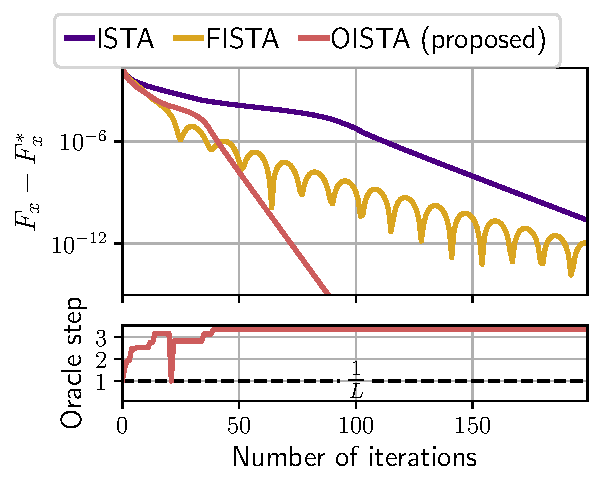
\includegraphics[width=.8\linewidth]{comparison_oista_ista}\\
        \myitem \parbox[t]{.8\linewidth}{But computing step-sizes at each iteration can be costly.}
    \end{column}
    \hskip-5pt
    \vrule width 1pt\hskip2pt
    \vrule width 1pt\hskip5pt
    \column{.5\textwidth}
    \textbf{Step LISTA (SLISTA)}\\[.5em]
    \myitem Restrict parameters to step-size:
    {\footnotesize
        \[\hskip-1em
        z^{(q + 1)} = \text{ST}\bigg(z^{(q)} - {\bf \color{blue!70}\alpha} D^\top(Dz^{(q)} - x), \lambda{\bf \color{blue!70}\alpha}\bigg)
        \]}%
    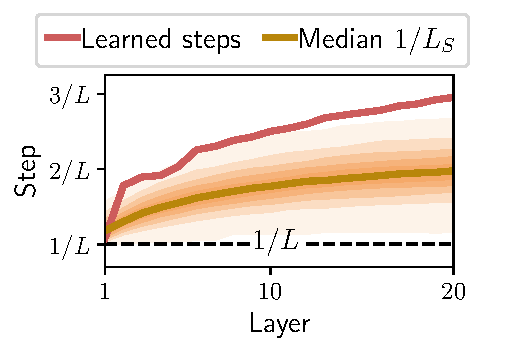
\includegraphics[width=.8\linewidth]{learned_steps}\\
    {\bf Theorem:} For any "converging" LISTA network, the weights tend toward step-size: $\frac{\alpha^*}{\theta^*}W^* = D$
\end{columns}
	\end{frame}


\begin{frame}[c]{Future work}
\begin{columns}[T]
    \column{.5\textwidth}%
\begin{itemize}
    \item {\bf Direct extension }\\[.5em]
    Extending our theorem to all LISTA network even without weights coupling.\\[1em]

    \item {\bf Optimal first layer}\\[.5em]
        Interpolation $D^\top$ and $D^\dagger$\\[1em]
    {\centering
    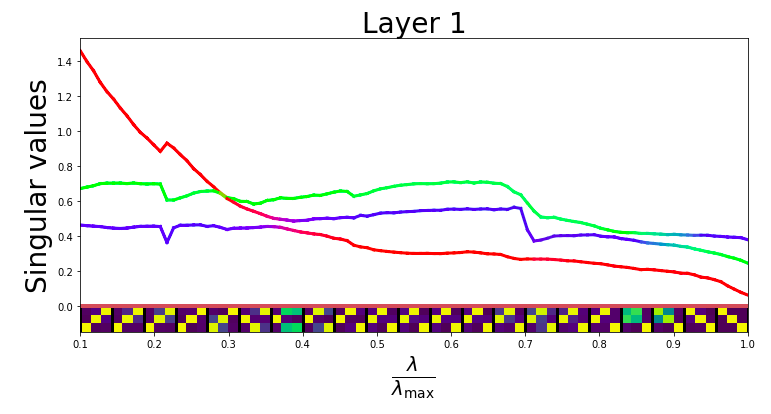
\includegraphics[width=.8\linewidth]{first_layer}\\[1em]}
\end{itemize}

    \column{.5\textwidth}
    \myitem \parbox[t]{.9\linewidth}{\raggedright
        {\bf Dictionary Learning}\\[.5em]
        Integrated model
        {\footnotesize\[
            \min_D \frac{1}{2}\|X - D\Phi_D(X)\|_2^2 + \lambda\|\Phi_D(X)\|_1
        \]}%
        Question:
        
\begin{itemize}
    \item[$\bullet$] How is it related to dictionary learning?
    \item[$\bullet$] Can we guarantee reconstruction properties.
\end{itemize}
        }
\end{columns}
\end{frame}

\end{document}
